\documentclass[12pt]{article}
\usepackage[utf8]{inputenc}

%% DEFINITIONS
\def\myname{Ethan Kessel}
\def\mytitle{ENGR 133 Individual Project Report}
\def\mysubtitle{LC4 - 2}

%% PACKAGES
\usepackage[margin = 1.0in]{geometry}   % Change margins
\usepackage{graphicx}                   % Pictures
\usepackage{subcaption}                 % Subfigures
\usepackage{fancyhdr}					% Fancy headers
\usepackage{nccmath}                    % https://tex.stackexchange.com/questions/520261/system-of-equations/520423
\usepackage{enumitem}% http://ctan.org/pkg/enumitem
\usepackage{tabularx}                   % better tables
\usepackage{tabulary}
\usepackage{amsfonts,amsmath,amssymb}	% Special symbols and tools
\usepackage{empheq}                     % loads mathtools, which loads amsmath
\usepackage{listings}                   % For code in document
\usepackage{lastpage}                   % Needed for "Pg. x of xx"
\usepackage[page,toc,titletoc,title]{appendix}   % Appendix package
\usepackage{tocloft}                    % ??
\usepackage{natbib}

% https://stackoverflow.com/questions/1966425/source-code-highlighting-in-latex#1985330
% \usepackage{fontspec}
% \usepackage{minted}
% \setsansfont{Calibri}
% \setmonofont{Consolas}

\usepackage{color}

%% SETUP
\pagestyle{fancy}
\fancyhead{}
\fancyfoot{}
\fancyhead[L]{{\bfseries\mytitle} -- \mysubtitle}
\fancyhead[R]{\myname}
\fancyfoot[R]{Pg. \thepage\ of \pageref{LastPage}}

%% https://tex.stackexchange.com/questions/83882/how-to-highlight-python-syntax-in-latex-listings-lstinputlistings-command
% Default fixed font does not support bold face
\DeclareFixedFont{\ttb}{T1}{txtt}{bx}{n}{8} % for bold
\DeclareFixedFont{\ttm}{T1}{txtt}{m}{n}{8}  % for normal
\DeclareFixedFont{\tti}{T1}{txtt}{it}{n}{8}  % for italics

% Custom colors
\definecolor{deepblue}{rgb}{0,0,0.5}
\definecolor{deepred}{rgb}{0.6,0,0}
\definecolor{deepgreen}{rgb}{0,0.5,0}
\definecolor{commentgray}{rgb}{0.6,0.6,0.6}

% Python style for highlighting
\newcommand\pythonstyle{\lstset{
language=Python,
numbers=left,
numberstyle=\ttm,
stepnumber=1,
basicstyle=\ttm,
commentstyle=\tti\color{commentgray},
otherkeywords={self},             % Add keywords here
keywordstyle=\ttb\color{deepblue},
emph={MyClass,__init__},          % Custom highlighting
emphstyle=\ttb\color{deepred},    % Custom highlighting style
stringstyle=\color{deepgreen},
frame=tb,                         % Any extra options here
showstringspaces=false,           % 
breaklines=true
}}


% Python environment
\lstnewenvironment{python}[1][]
{
\pythonstyle
\lstset{#1}
}
{}

% Python for external files
\newcommand\pythonexternal[2][]{{
\pythonstyle
\lstinputlisting[#1]{#2}}}

% Python for inline
\newcommand\pythoninline[1]{{\pythonstyle\lstinline!#1!}}

% \lstset
% { %Formatting for code in appendix
%     language=Python,
%     basicstyle=\footnotesize,
%     numbers=left,
%     stepnumber=1,
%     showstringspaces=false,
%     tabsize=1,
%     breaklines=true,
%     breakatwhitespace=false,
% }

\graphicspath{ {./assets/} }

\begin{document}
\begin{titlepage}
\vspace*{1in}
\centering

{\bfseries\LARGE \mytitle \par}
\vspace{0.5in}
{\large \mysubtitle \par}
\vfill
{\Large \myname \par}
\vspace{0.5in}
Group Members:\\
Jasper Jones, Nathan Yakupkovic, David Kopp\par
\vfill
{\scshape\Large Purdue University\par}
\vspace{0.5in}
{\large \today\par}

\vspace*{1.5in}
\thispagestyle{empty}
\end{titlepage}

\tableofcontents
\listoffigures
\listoftables
\thispagestyle{empty}
\clearpage

\setcounter{page}{1}

\section{Introduction}
This project will be exploring the electrical behavior of an astable multivibrator oscillator circuit making use of an operational amplifier using Python and the integrate module of scipy. In a world where microcontrollers allow for easy control of electrical outputs and small devices, more elegant electromechanical solutions have fallen to the wayside of the entry-level hobbyist or engineer. Although my first choice for my major is Aeronautical and Astronautical Engineering, I still have a passion for the electronics that power modern avionics and our daily lives, and want to gain a better understanding of the operation of circuits. This semester, I took an electronics workshop through the Office of Professional Practice, during which we constructed a circuit to blink an LED using nothing but passive components and an op-amp IC.  Such a circuit is exceedingly easy to implement using an Arduino microcontroller, but the task can be achieved just as effectively with a much more elegant solution that is cheap and does not require a computer unnecessarily. A reconstruction of the circuit I constructed is shown in Figure \ref{fig:breadboard}.

\begin{figure}[h!]
\centering
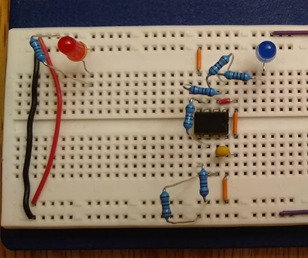
\includegraphics[width=0.6\textwidth]{breadboard.png}
\caption{Op-Amp Circuit Assembled on a Solderless Breadboard}
\label{fig:breadboard}
\end{figure}

During the assignment where I was building this circuit, I did not have a good intuition as to how it functioned. I decided that I would attempt to model the circuit in Python using the integrate module of scipy to solve a differential system numerically. I had to perform some research into the behavior of operational amplifiers as well as apply knowledge gained from my participation in PHYS 272 this semester to come to a solution. I then also compared my theoretical results to reality using an oscilloscope I have on-hand at home, which showed some interesting results.

\section{Problem Analysis}
\subsection{Circuit Diagram}
The first step to analyzing the problem was to draw a circuit diagram. One had been provided as part of the workshop however it did not fully match the circuit that was actually built and furthermore did not let me intuitively understand what was occurring in the circuit. I utilized Autodesk EAGLE to redraw the circuit diagram of my circuit, which is shown in Figure \ref{fig:circuit_diagram}.

\begin{figure}[h!]
\centering
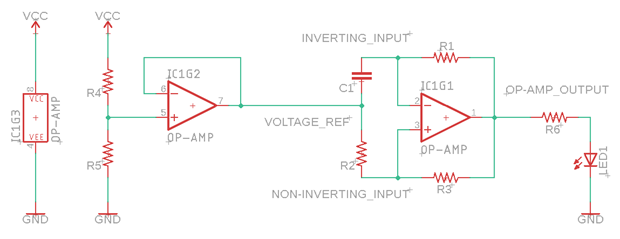
\includegraphics[width=1.0\textwidth]{circuit_diagram.png}
\caption{Autodesk EAGLE Circuit Diagram}
\label{fig:circuit_diagram}
\end{figure}

The circuit has two main functional parts, each using a singular operational amplifier. On the left is what is known as a voltage follower; it is an amplifier set up with negative feedback such that it produces unity gain. What this is useful for is maintaining a specific voltage at a  node regardless of the current drawn. The input of this voltage follower is connected to a voltage divider (consisting of resistors \texttt{R4} and \texttt{R5}), and copies the voltage produced at that node to the output. On the right is the astable multivibrator oscillator. It consists of a voltage divider and an RC circuit, connected between a constant reference voltage produced by the voltage follower and the op-amp’s output. Further explanation of how this produces an oscillating signal will be discussed once the behavior of an op-amp and the circuit components are discussed.

\subsection{Operational Amplifier Behavior}
Early in the research for this project I needed to find a way to model the behavior of an operational amplifier. Fortunately, this ended up being very simple. I was able to find a textbook chapter online \cite{springerEE} that provided an excellent explanation of the material, however the chapter has since become pay-for and I can no longer access the material on the page, so I will continue using material from my notes. The model of an operational amplifier is quite simple and shown in Equation \ref{eq:op-amp}.

\begin{spreadlines}{0.5ex}
\begin{equation} \label{eq:op-amp}
v_\text{out} =
\begin{dcases}
V_{CC} & \text{if}\; v_\text{out} > V_{CC}\\
A\left(v^+ - v^-\right) + \frac{V_{CC} + V_{EE}}{2} & \text{if}\; V_{EE} \leq v_\text{out} \leq V_{CC} \\
V_{EE} & \text{if}\; v_\text{out} < V_{EE}\\ 
\end{dcases}
\end{equation}
\end{spreadlines}

These equations show that the output of the operational amplifier is linearly proportional to the differential input voltage $(v^+ - v^-)$ but is capped between the voltages supplied to the op-amp. Visually, this is shown in Figure \ref{fig:op-amp_fn}.

\begin{figure}[h!]
\centering
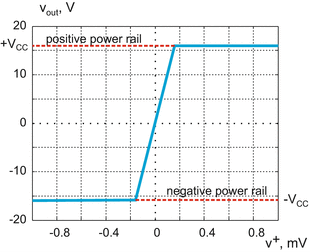
\includegraphics[width=0.5\textwidth]{op-amp_func.png}
\caption{Output of an Operational Amplifier vs. Differential Input Voltage}
\label{fig:op-amp_fn}
\end{figure}

Because the amplification value $A$ is often very high (on the order of $10^6$ or more), an operational amplifier in open-loop operation is almost always saturated at the voltages supplied, producing a digital signal. In this sense, the op-amp is a voltage comparator, producing a positive output when $v^+$ is greater than $v^-$, and a negative output when the opposite is true. However, it is important to note that this is ideal behavior. In reality, the chapter noted that the output is often a bit short of completely reaching supplied voltages. For my purposes I ignored this and approximated the op-amp as ideal. Furthermore, a real op-amp has several other non-ideal characteristics, such as a non-infinite impedance between the two inputs, and a nonzero impedance of the output. The effects of these are negligible and vastly complicate the modeling, so I will approximate them away as well.\par

In the specifications for operational amplifiers, the unitless amplification value $A$ is not given and instead a gain in decibels is specified. The formula to convert between decibels and amplification is rather simple and is shown in Equation \ref{eq:decibel_amp}.
\begin{align} \label{eq:decibel_amp}
    \text{Gain} = 20 \text{dB} \cdot \log_{10}A \quad \leftrightarrow \quad A = 10^{\left(\frac{\text{Gain}}{20 \text{dB}}\right)}
\end{align}

\subsection{Mathematical Analysis of Circuit Dynamics}
The oscillator shown in Figure \ref{fig:circuit_diagram} consists of two common electrical devices, a voltage divider and an RC circuit. The op-amp measures the voltage of the voltage divider with its non-inverting input, and the voltages of the RC circuit with its inverting input. Both the voltage divider and RC circuit are connected across the regulated voltage reference and the operational amplifier output. The voltage at the non-inverting input, as created by the voltage divider, is given by Equation \ref{eq:volt_divide}.

\begin{align} \label{eq:volt_divide}
v^+ = \frac{\left(v_\text{out} - v_\text{ref}\right)R_2}{R_2 + R_3} + v_\text{ref}
\end{align}

The equations for the RC circuit section are a bit more complicated and involve differential equations. Using Kirchhoff's Voltage Law, Ohm's Law, and the equation for the voltage drop of a capacitor, Equation \ref{eq:diffeq} is obtained.

\begin{align} \label{eq:diffeq}
\Delta V_\text{capacitor} + \Delta V_\text{resistor} &= v_\text{out} - v_\text{ref} \nonumber\\
\frac{Q}{C} + IR_1 &= v_\text{out} - v_\text{ref} \nonumber\\
\frac{Q}{C} + \dot{Q}R_1 &= v_\text{out} - v_\text{ref} \nonumber\\
\dot{Q} &= \frac{v_\text{out} - v_\text{ref}}{R_1} - \frac{Q}{R_1C}
\end{align}

\noindent
Using the charge on the capacitor $Q$ the voltage at the inverting input can be found as in Equation \ref{eq:volt_RC}.

\begin{align} \label{eq:volt_RC}
v^- &= v_\text{ref} + \Delta V_\text{capacitor} \nonumber\\
    &= v_\text{ref} + \frac{Q}{C}
\end{align}

\noindent
All of these may be combined into a large system of equations (Equation \ref{eq:system}).

\begin{spreadlines}{0.5ex}
\begin{equation} \label{eq:system}
\begin{dcases}
\dot{Q} &= \frac{v_\text{out} - v_\text{ref}}{R_1} - \frac{Q}{R_1C}\\
v^- &= v_\text{ref} + \frac{Q}{C}\\
v^+ &= \frac{\left(v_\text{out} - v_\text{ref}\right)R_2}{R_2 + R_3} + v_\text{ref}\\
v_\text{out} &=
    \begin{dcases}
    V_{CC} & \text{if}\; v_\text{out} > V_{CC}\\
    A\left(v^+ - v^-\right) + \frac{V_{CC} + V_{EE}}{2} & \text{if}\; V_{EE} \leq v_\text{out} \leq V_{CC} \\
    V_{EE} & \text{if}\; v_\text{out} < V_{EE}\\ 
    \end{dcases}
\end{dcases}
\end{equation}
\end{spreadlines}

Although a number of approximations and simplifications were made, the resulting system is still quite complicated and ugly, with piecewise components and circular references. Fortunately, solving such a system numerically alleviates the majority of these issues.

\subsection{Numerical Solution}
Since $v_\text{out}$ depends on $v^+$ and $v^-$, and similarly $v^+$ and $v^-$ depend on $v_\text{out}$, an analytical solution is difficult. Using a numerical approach allows for a rather natural solution. The voltage at each of op-amp inputs ($v^+$ and $v^-$) may be calculated using the values from the previous time step and then fed into the op-amp function for the current time step. This resolves the issue with the circular references complicating the equation, and should be accurate assuming a small enough time step is used.\par 
Such a solution was implemented in Python using the \texttt{scipy.integrate.ode} module. When run, the following results (Figure \ref{fig:sim1}) were produced with the constants shown in Table \ref{tab:consts}.

\begin{spreadlines}{1ex}
\begin{table}[h!]
    \centering
    \caption{Constant Parameters for Simulation}\vspace{2mm}
    \begin{tabular}{c|rl}
    Constant &  \multicolumn{2}{c}{Value}\\
    \hline
    $C$         &   $1\cdot10^{-6}$     & F\\
    $R_1$       &   $100\cdot10^3$      & $\Omega$\\
    $R_2$       &   $10\cdot10^3$       & $\Omega$\\
    $R_3$       &   $10\cdot10^3$       & $\Omega$\\
    Gain        &   100                 & dB\\
    $V_{CC}$    &   5.0                 & V\\
    $V_{EE}$    &   0.0                 & V\\
    $v_\text{ref}$ & 2.5                & V\\
    $t_0$       &   0.0                 & sec\\
    $t_f$       &   1.0                 & sec\\
    $\Delta t$  &   0.001               & sec
    \end{tabular}
    \label{tab:consts}
\end{table}
\end{spreadlines}

\begin{figure}[h!]
\centering
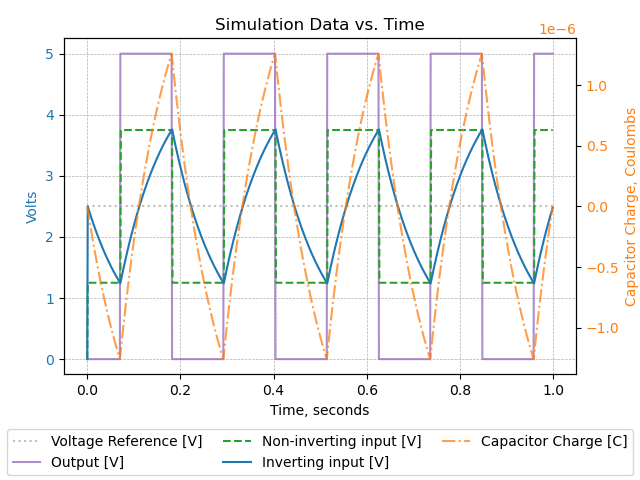
\includegraphics[width=0.75\textwidth]{Simulation_1.png}
\caption{Simulation Results using Constants in Table \ref{tab:consts}}
\label{fig:sim1}
\end{figure}

\subsection{Analysis of Oscillation Parameters} \label{sec:oscillate_params}
The method of oscillation becomes apparent looking at Figure \ref{fig:sim1}. The op-amp output is constantly saturated at either $V_{CC}$ or $V_{EE}$, and the voltage divider creates a voltage in between $v_\text{out}$ and $v_\text{ref}$ at the non-inverting input. The voltage at the inverting input changes continually as the capacitor charges and discharges; the voltage it produces at the inverting input constantly chases the voltage at the non-inverting input due to the polarization of $v_\text{out} - v_\text{ref}$, and upon reaching the non-inverting input the output swaps and the process repeats in the opposite direction. Using this observation, it is possible to derive analytical solutions for the time behavior of the oscillator.\par
The initial step is to identify a solution to the differential equation in Equation \ref{eq:diffeq}. There is a well-known solution for an RC circuit and it is shown in Equation \ref{eq:capacitor_soln}.
\begin{align} \label{eq:capacitor_soln}
    \frac{Q}{C} = v_\text{capacitor} = v_\text{applied} \left( 1 - e^{-\frac{t}{R_1C}} \right)\\
    \text{where}\ v_\text{applied} = v_\text{out} - v_\text{ref} \nonumber
\end{align}
\par
To find the time elapsed for when the voltage output is high, consider a segment of time from when the voltage output just switched from low ($V_{EE}$) to high ($V_{CC}$). What needs to be found is the time taken for the inverting input voltage to charge from the non-inverting input voltage when the output is low (Equation \ref{eq:high_t_start}) to the non-inverting input voltage when the voltage is high (Equation \ref{eq:high_t_finish}).

\begin{align}
\left. v^- \right|_{t=t_s} &= \left. v^+ \right|_{t=t_s}\nonumber\\
\left. v_\text{ref} + \frac{Q}{C} \right|_{t=t_s} &= \left. \frac{\left(v_\text{out} - v_\text{ref}\right)R_2}{R_2 + R_3} + v_\text{ref} \right|_{t=t_s}\nonumber\\
\left. \left( v_\text{out} - v_\text{ref} \right)\left( 1 - e^{-\frac{t}{R_1C}} \right) \right|_{t=t_s} &= \left. \frac{\left(v_\text{out} - v_\text{ref}\right)R_2}{R_2 + R_3} \right|_{t=t_s}\nonumber\\
\label{eq:high_t_start}
\left( V_{CC} - v_\text{ref} \right)\left( 1 - e^{-\frac{t_s}{R_1C}} \right) &= \frac{\left(V_{EE} - v_\text{ref}\right)R_2}{R_2 + R_3}\\
\nonumber\\
\left. v^- \right|_{t=t_f} &= \left. v^+ \right|_{t=t_f}\nonumber\\
\label{eq:high_t_finish}
\left( V_{CC} - v_\text{ref} \right)\left( 1 - e^{-\frac{t_f}{R_1C}} \right) &= \frac{\left(V_{CC} - v_\text{ref}\right)R_2}{R_2 + R_3}
\end{align}

\noindent
The high output time period $\Delta t_\text{high}$ is found from the difference $t_f - t_s$ (Equation \ref{eq:t_high}).

\begin{align}
\left( V_{CC} - v_\text{ref} \right)\left( 1 - e^{-\frac{t_s}{R_1C}} \right) &= \frac{\left(V_{EE} - v_\text{ref}\right)R_2}{R_2 + R_3}\nonumber\\
1 - e^{-\frac{t_s}{R_1C}} &= \frac{\left(V_{EE} - v_\text{ref}\right)R_2}{\left(R_2 + R_3\right)\left( V_{CC} - v_\text{ref} \right)}\nonumber\\
e^{-\frac{t_s}{R_1C}} &= 1 - \frac{\left(V_{EE} - v_\text{ref}\right)R_2}{\left(R_2 + R_3\right)\left( V_{CC} - v_\text{ref} \right)}\nonumber\\
t_s &= - R_1C \ln \left[1 - \frac{\left(V_{EE} - v_\text{ref}\right)R_2}{\left(R_2 + R_3\right)\left( V_{CC} - v_\text{ref} \right)}\right]\nonumber\\
\nonumber\\
t_f &= - R_1C \ln \left[1 - \frac{\left(V_{CC} - v_\text{ref}\right)R_2}{\left(R_2 + R_3\right)\left( V_{CC} - v_\text{ref} \right)}\right]\nonumber\\
    &= - R_1C \ln \left[1 - \frac{R_2}{R_2 + R_3}\right]\nonumber
\end{align}

\begin{align} \label{eq:t_high}
\Delta t_\text{high} = t_f - t_s &= R_1C \left(\ln \left[1 - \frac{\left(V_{EE} - v_\text{ref}\right)R_2}{\left(R_2 + R_3\right)\left( V_{CC} - v_\text{ref} \right)}\right] - \ln \left[1 - \frac{R_2}{R_2 + R_3}\right] \right)
\end{align}

\noindent
By a similar computation, the low output time period $\Delta t_\text{low}$ may be found (Equation \ref{eq:t_low}).

\begin{align} \label{eq:t_low}
\Delta t_\text{low} &= R_1C \left(\ln \left[1 - \frac{\left(V_{CC} - v_\text{ref}\right)R_2}{\left(R_2 + R_3\right)\left( V_{EE} - v_\text{ref} \right)}\right] - \ln \left[1 - \frac{R_2}{R_2 + R_3}\right] \right)
\end{align}

If I place some constraints on the constant parameters of these equations, it is possible to solve for a desired $R_1C$ time constant given a desired period or frequency. If I constrain $R_2 = R_3$ and that $v_\text{ref}$ is between $V_{CC}$ and $V_{EE}$ such that $\left(V_{EE} - v_\text{ref}\right) = - \left(V_{CC} - v_\text{ref}\right)$, the equation greatly simplifies yielding Equations \ref{eq:RC_period} and \ref{eq:RC_freq}.

\begin{align}
\Delta t_\text{high} = \Delta t_\text{low} = R_1C \left(\ln \left[\frac{3}{2}\right] - \ln \left[\frac{1}{2}\right] \right) = R_1C\ln 3 \nonumber
\end{align}

\begin{align}
\label{eq:RC_period}
T = \Delta t_\text{high} + \Delta t_\text{low} = 2 R_1C\ln 3 \quad \rightarrow \quad R_1C &= \frac{T}{2\ln 3}\\
\label{eq:RC_freq}
f = \frac{1}{T} = \frac{1}{2 R_1C\ln 3} \quad \rightarrow \quad  R_1C &= \frac{1}{2f\ln 3}
\end{align}

\section{Program Details}
The Python script I developed for this project comes with three main execution sections:
\begin{enumerate}[label*=(\roman*)]
    \item \label{it:load} Load in the simulation constant values.
    \item \label{it:sim} Simulate the system using \texttt{scipy.integrate.ode}.
    \item \label{it:out} Output the simulation results and other calculated statistics.
\end{enumerate}

\subsection{Section \ref{it:load} -- Load Constants} \label{sec:load}
All user input occurs in Section \ref{it:load} with loading the simulation constants. There are three primary options for user input in this section:
\begin{enumerate}
    \item \label{it:default} Load default constant values.
    \item \label{it:json} Load constants from a \texttt{.json} file.
    \item \label{it:manual} Load constants via manual user input.
    \begin{enumerate}
        \item \label{it:man_all} Input all constants manually.
        \item \label{it:man_RC} Calculate RC value given period or frequency.
    \end{enumerate}
\end{enumerate}
Options \ref{it:default} and \ref{it:json} are similar as they both load the constants from a \texttt{.json} file. Option \ref{it:json} allows the user to specify a path to a \texttt{.json} constants file (or just the name of the file if in the same directory as the scripts). The input is validated to make sure it is a \texttt{.json} file and has all of the necessary constant parameters (in a user-defined function). Option \ref{it:default} simply bypasses the user input for the file path used in Option \ref{it:json} and uses the \texttt{.json} defaults file that is specified in the code. Option \ref{it:manual} also uses the same defaults file as Option \ref{it:default}, but will allow the user to override the constant parameters with their own value. Any input for an entry that is left blank or invalid is left as the default in this case. Suboption \ref{it:man_all} allows the user to input parameters for all of the constant values (see Table \ref{tab:consts} for the constants used). Suboption \ref{it:man_RC} allows the user to specify a desired period or frequency and calculate the needed RC time constant as in Section \ref{sec:oscillate_params} using Equation \ref{eq:RC_period}. The program then calculates the correct resistor and capacitor pairing given either a fixed resistance or capacitance. As noted in Section \ref{sec:oscillate_params}, certain assumptions must be made for this calculation to be performed, and as a result the program limits what other constant values may be defined in this case, with the rest being kept as the defaults. The permitted values are shown in Table \ref{tab:RC_allowed_consts}.

\begin{spreadlines}{1ex}
\begin{table}[h]
    \centering
    \caption{Allowed User-Changeable Constant Parameters for RC Time Constant Calculation}\vspace{2mm}
    \begin{tabular}{c|c}
    Constant &  Units\\
    \hline
    Gain        & dB\\
    $t_0$       & sec\\
    $t_f$       & sec\\
    $\Delta t$  & sec
    \end{tabular}
    \label{tab:RC_allowed_consts}
\end{table}
\end{spreadlines}
\noindent
At the end of this section the constant parameters are redisplayed for the user's reference.

\subsection{Section \ref{it:sim} -- Run Simulation}
In Section \ref{it:sim}, the simulation is prepared and run. A user-defined function is used to produce a function object that behaves as specified in Equation \ref{eq:op-amp}, and several \texttt{numpy} arrays are prepared to store the simulation data over time. The time steps array is made first using the \texttt{arange} function, and all other data series are made using \texttt{zeros\_like} to match. The differential equation (Equation \ref{eq:diffeq}) is defined to take in the system state and output $\frac{dQ}{dt}$ in accordance with what is required by \texttt{scipy.integrate.ode}, and an ODE solver object is created and initialized with the initial values to solve the IVP. The system is then run while successful until the simulation end time is reached using the equations in Equation System \ref{eq:system}.

\subsection{Section \ref{it:out} -- Output Results}
Finally in Section \ref{it:out} output is produced for the user.  The oscillation parameters (frequency, period, duty cycle, high period, and low period) are calculated using Equations \ref{eq:t_high} and \ref{eq:t_low} in a user-defined function, then displayed to the console. A graph is then created using \texttt{matplotlib} to show the evolution of the system value over time. Lastly, the simulation values are exported to an \texttt{output.csv} file for future reference.

\subsection{User-Defined Functions}
The Python program makes use of five user-defined functions for various purposes. Their uses are briefly summarized in Table \ref{tab:udfs}.

\begin{table}[h]
    \centering
    \caption{User-Defined Functions Used in the Simulation Code}\vspace{2mm}
    
    \renewcommand\tabularxcolumn[1]{m{#1}}% for vertical centering text in X column
    \newcolumntype{L}[1]{>{\hsize=#1\raggedright\arraybackslash}X}%
    
    \begin{tabularx}{\linewidth}{l|L{0.8in}|L{0.6\linewidth}}
    UDF Name (Arguments)   & \centering Returns    & Summary\\
    \hline
    \texttt{validateJSONconstants(path)} & none & Checks a \texttt{.json} file specified to make sure it has the necessary parameters. Raises an exception to be handled if the file is missing parameters, passes otherwise.\\
    \hline
    \texttt{dBtoAmp(decibels)} & unitless amplitude & Converts decibels to amplitude as shown in Equation \ref{eq:decibel_amp}.\\
    \hline
    \texttt{makeOpAmpFunc(gain, vcc, vee)} & function object & Generates a function object that behaves like Equation \ref{eq:op-amp}.\\
    \hline
    \texttt{userInputCalculate(defaults\_fpath)} & constants namespace \texttt{c} & Gets user input for simulation constant parameters or calculates parameters based on desired frequency/period.\\
    \hline
    \texttt{computeFrequencyParams(c)} & \texttt{tuple} of values & Determines the frequency, period, duty cycle, high period, and low period using Equations \ref{eq:t_high} and \ref{eq:t_low} based on the constant parameters in the namespace \texttt{c}.\\
    \end{tabularx}
    \label{tab:udfs}
\end{table}
\noindent
In the main script a \texttt{dQ\_dt(t, Q, consts, Vout)} function is defined. This is required for the ODE solver to function and is only used for that purpose.

\subsection{Use of \texttt{lambda} Declaration}
In Python the keyword \texttt{lambda} is used to declare anonymous function objects. It gets its name from \emph{Lambda Calculus}, which is a mathematical system for expressing computation based on binding abstracted functions to variables. Unlike regular functions in Python which are created with the \texttt{def} keyword followed by a function name, \texttt{lambda} functions are never defined with a name, hence the term ``anonymous''. \texttt{lambda} functions are incredibly useful as they allow for the definition of simple functions on the fly that can be assigned to variables or passed into functions expecting a function input. The following listing demonstrates how a \texttt{lambda} was used to pass the constructor for \texttt{simpleNamespace} into the \texttt{.json} loader function. It specifies how the produced object (a \texttt{dict} type) should be fed into the constructor.

\pythonexternal[linerange={105-105}, numbers=none, title={Example of a \texttt{lambda} Used to Pass a Function Into Another Function}]{./PythonCode/ENGR133_Project_circuitSim_ekessel.py}

\noindent
A \texttt{lambda} was also used in \texttt{makeOpAmpFunc} to create a function object.

\pythonexternal[linerange={68-72}, numbers=none, title={Example of a \texttt{lambda} Used to Create an Anonymous Function}]{./PythonCode/ENGR133_Project_circuitSim_funcs_ekessel.py}

\noindent
They also saw use in the \texttt{userInputCalculate} function to help with unit conversion. By assigning the resultant function object to a variable I was able to make the code accept different input units depending on what the user selected but still produce the correct output without having to add extra logic to process the user's numerical input.

\pythonexternal[linerange={121-131}, numbers=none, title={A \texttt{lambda} Used to Create Different Functional Behaviors Depending on User Input}]{./PythonCode/ENGR133_Project_circuitSim_funcs_ekessel.py}
\pythonexternal[linerange={147-157}, numbers=none]{./PythonCode/ENGR133_Project_circuitSim_funcs_ekessel.py}

\section{Comparison to Actual Circuit}
With access to an oscilloscope at home, I was able to compare my simulation results to empirical data. With the circuit constructed as in Figure \ref{fig:breadboard}, I connected it to an oscilloscope and digital power supply as shown in Figure \ref{fig:oscope_setup}.

\begin{figure}[h!]
\centering
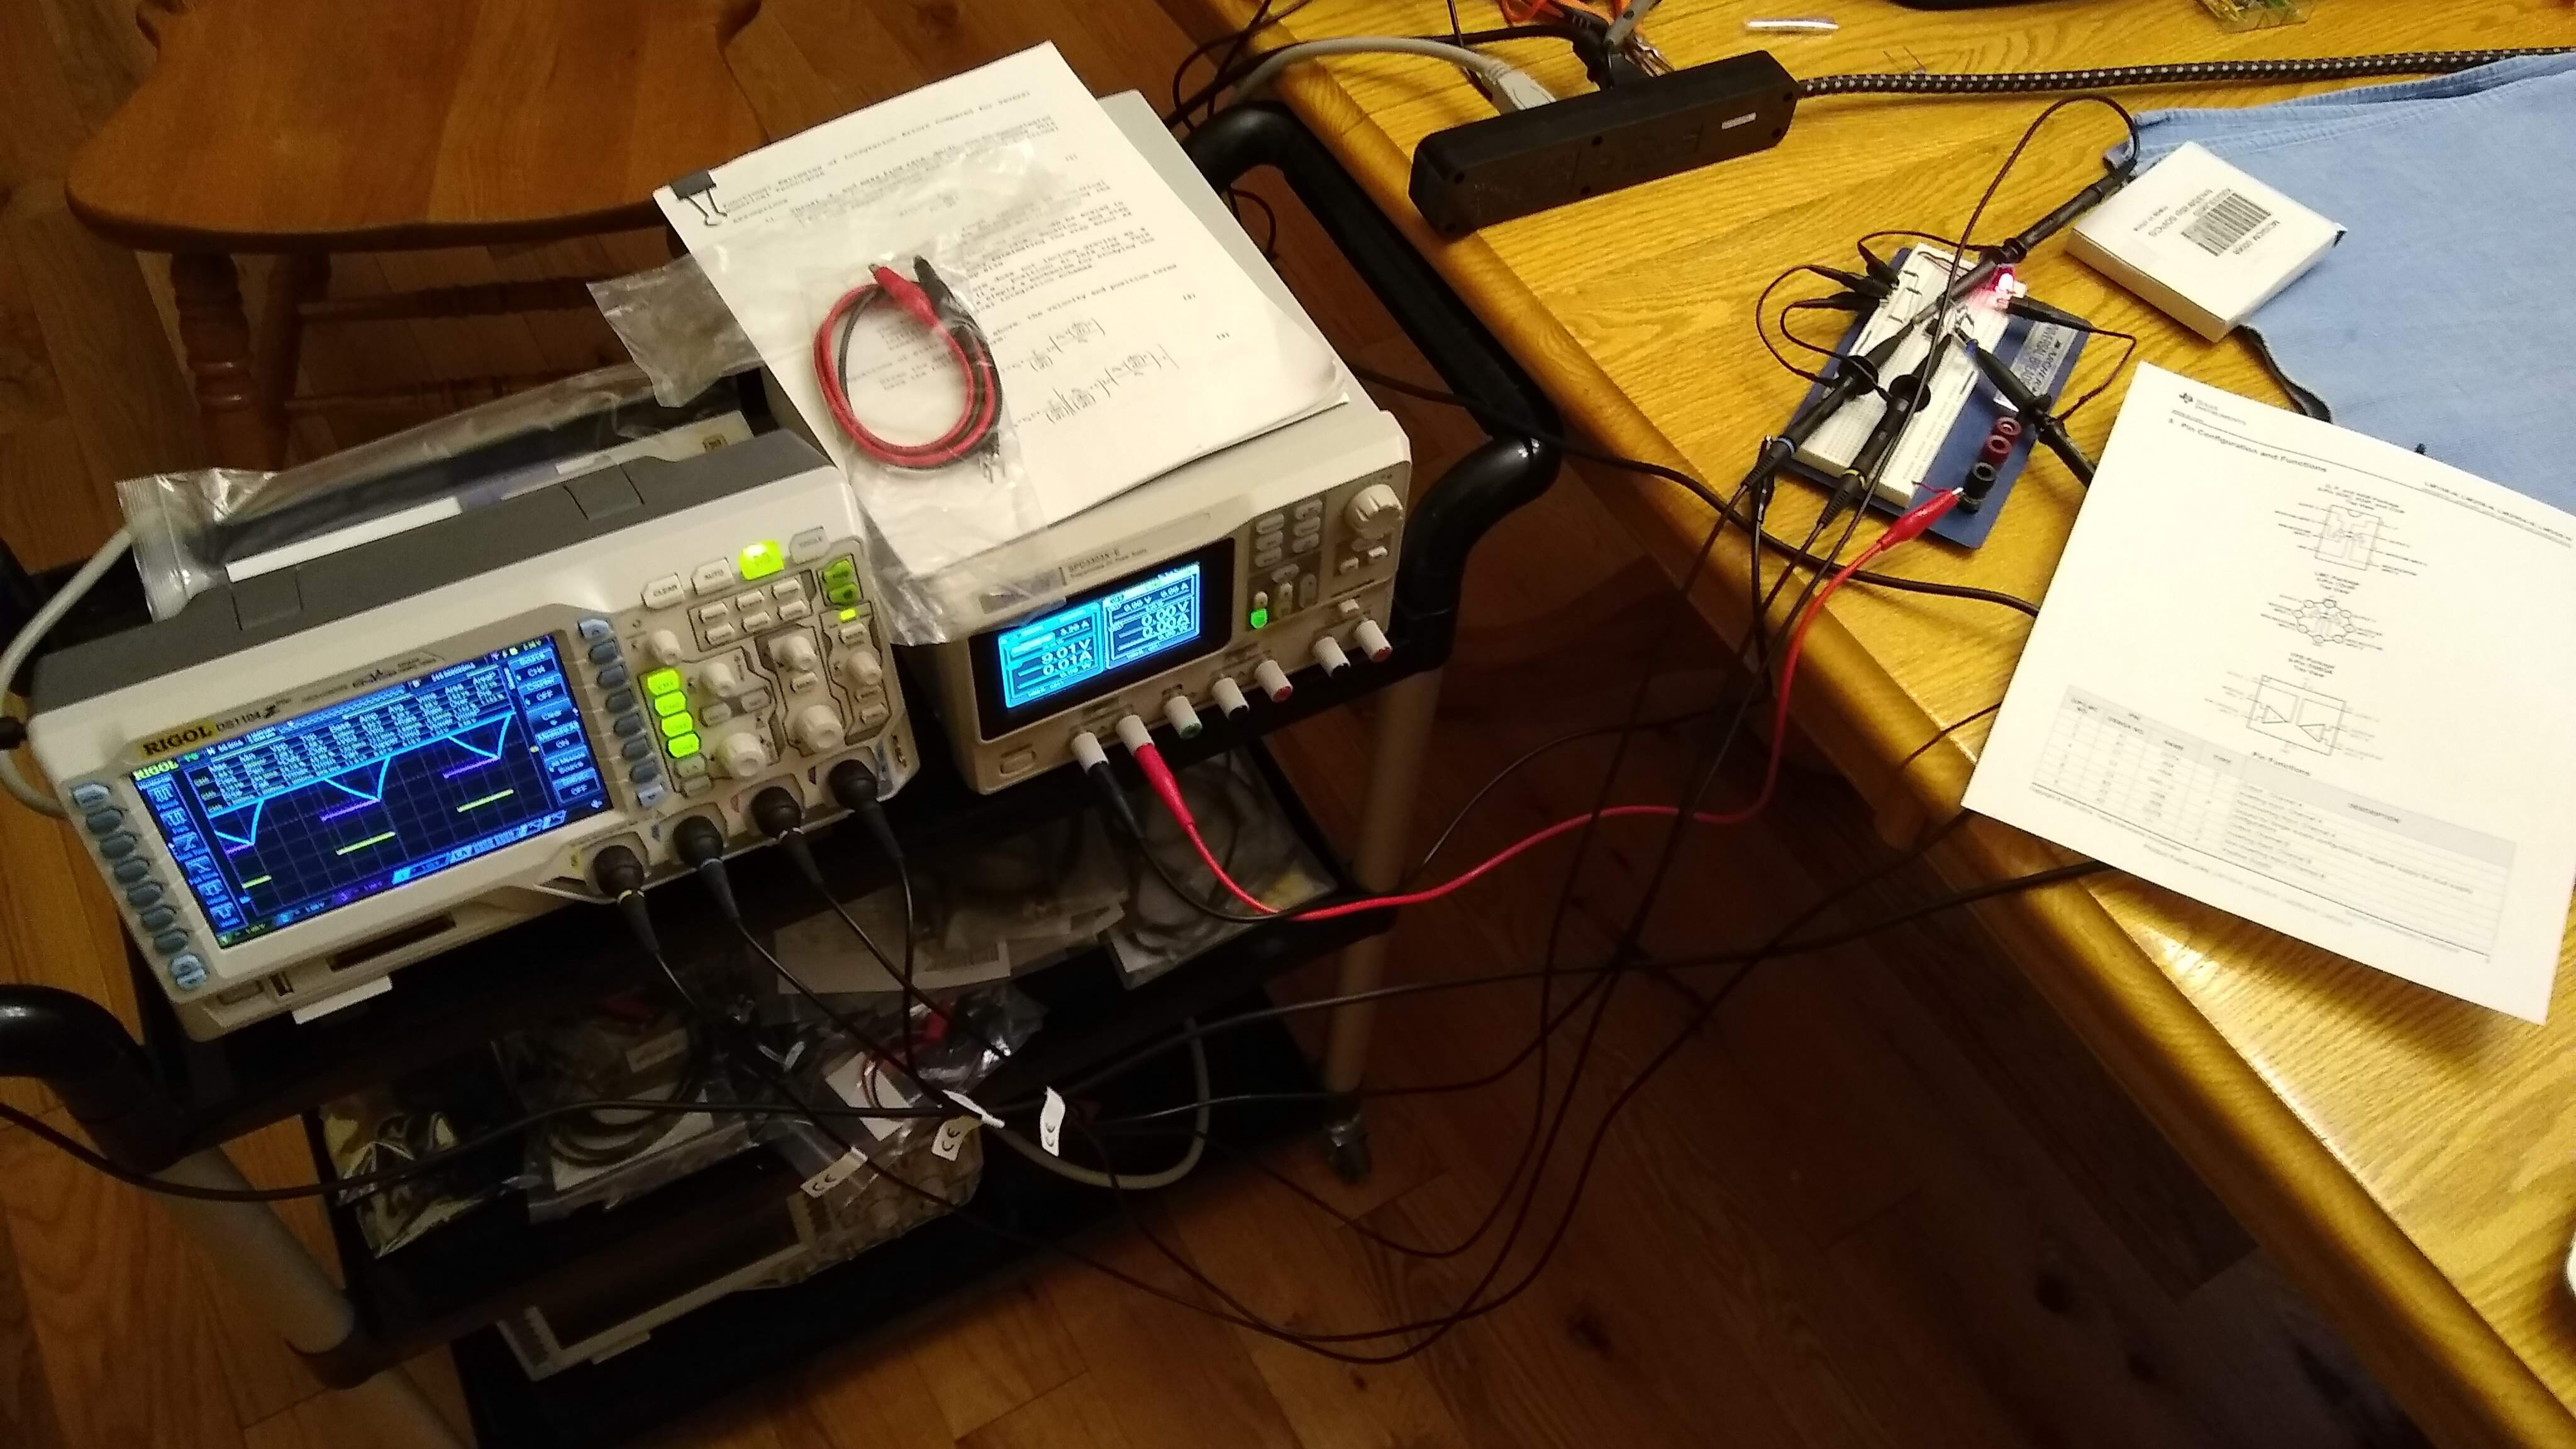
\includegraphics[width=1.0\textwidth]{Oscope_setup.jpg}
\caption{Oscillator Circuit as Connected to Oscilloscope}
\label{fig:oscope_setup}
\end{figure}

\noindent
I performed data collection of the operation of the actual circuit, which revealed interesting results which deviated from my predictions. Graphs produced from the oscilloscope are shown in Figure \ref{fig:oscope_data}. Components with values matching those specified in Table \ref{tab:consts} were used; resistors were accurate to within 1\% and an LM358-N operational amplifier was used.

\clearpage
\begin{figure}[h!]
\centering
\begin{subfigure}{\textwidth}
  \centering
  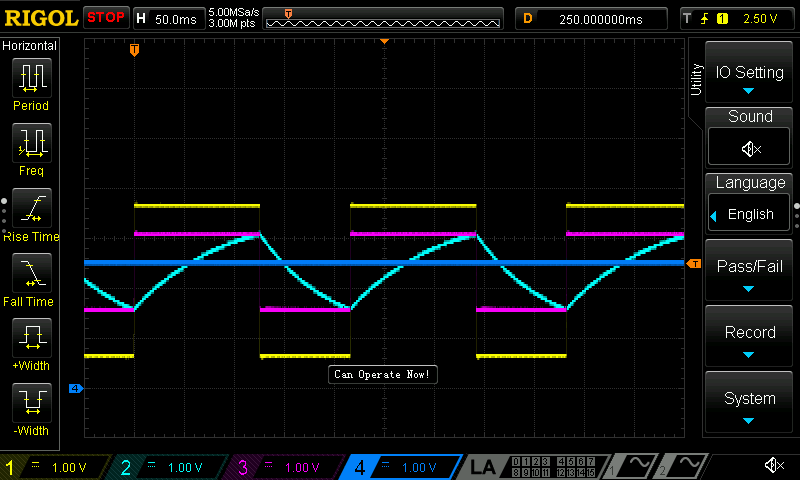
\includegraphics[width=0.8\linewidth]{ethan_screen_capture.png}
  \caption{Screenshot Produced by Oscilloscope}
  \label{fig:oscope_screenshot}
\end{subfigure}\\
\begin{subfigure}{\textwidth}
  \centering
  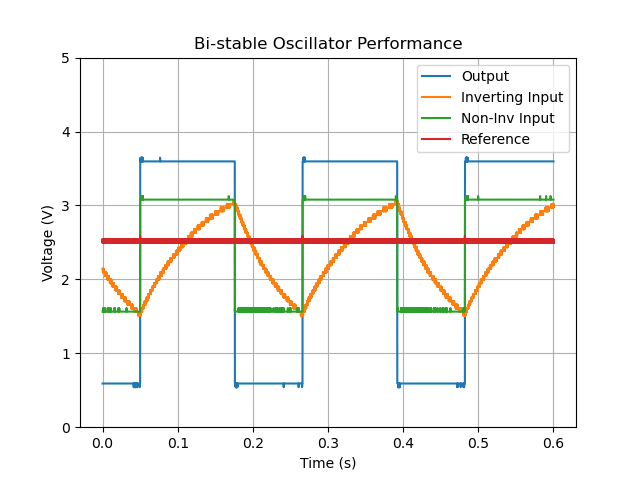
\includegraphics[width=1.0\linewidth]{ethan_plot.png}
  \caption{Graph Produced from Exported Data}
  \label{fig:oscope_graph}
\end{subfigure}
% \centering
% 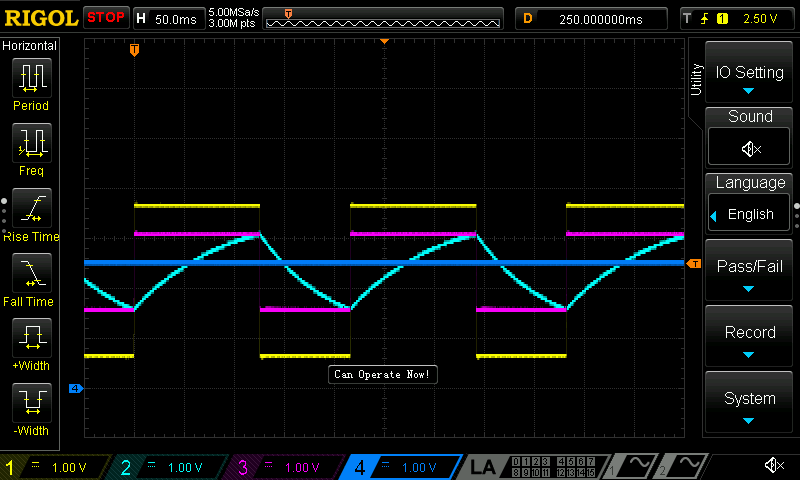
\includegraphics[width=1.0\textwidth]{ethan_screen_capture.png}\\
% 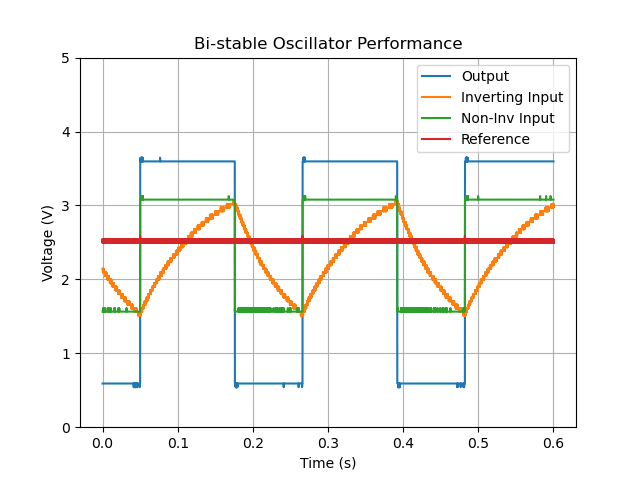
\includegraphics[width=1.0\textwidth]{ethan_plot.png}
\caption{Data Collected from the Oscilloscope}
\label{fig:oscope_data}
\end{figure}
\clearpage

The resulting graphs look remarkably similar to what my simulation showed, however what was immediately obvious was that the output produced was not a square wave with a 50\% duty cycle, and the frequency was off from what was expected. Table \ref{tab:expected_vs_real} shows a comparison between the expected and measured values.

\begin{spreadlines}{1ex}
\begin{table}[h]
    \centering
    \caption{Expected and Measured Values of Circuit Using Constants in Table \ref{tab:consts}}\vspace{2mm}
    \begin{tabular}{l|c|c}
    & Expected & Measured\\
    \hline
    Frequency (Hz) & 4.551 & 4.619 \\
    Period (sec) & 0.220 & 0.217 \\
    Duty Cycle & 50.0\% & 58.0\%\\
    High Period (sec) & 0.110 & 0.126 \\
    Low Period (sec) & 0.110 & 0.091 \\
    Output Max. (V) & 5.0 & 3.621\\
    Output Min. (V) & 0.0 & 0.560 \\
    Oscillator Ref. (V) & 2.5 & 2.541 \\
    \end{tabular}
    \label{tab:expected_vs_real}
\end{table}
\end{spreadlines}

After analyzing these data, I noticed that the outputs of the operational amplifier were not reaching $V_{CC}$ = 5.0V and $V_{EE}$ = 0.0V as expected, while $v_\text{ref}$ was reasonably close to the expected 2.5V. Notably, the operational amplifier was reaching the saturation voltages different distances from the expected output on either end. The low output was only 0.56V too high, but the high output was nearly 1.38V too low. As a result, the differential voltage $v_\text{out} - v_\text{ref}$ applied to the RC circuit varied in magnitude between the high and low periods which threw off the periods of each oscillation cycle. Since the magnitude of the differential voltage applied is greater in the low state than the high state, the capacitor charges faster in this state and the period is shortened versus the high state.
\par
This deviation from the expected results somewhat invalidates the simple model assumption (Equation \ref{eq:op-amp}) that I had used to make my simulation and predictions. The uneven output voltage offset from $V_{CC}$ and $V_{EE}$ are not something that my simulator addresses so the results produced are not completely accurate to reality. Furthermore, my attempts to find this phenomenon documented in the LM358-N's specification sheet did not turn up anything, so attempting to correct my model is not something I shall be able to do in the immediate future. However, recalling the assumptions made for calculations in Section \ref{sec:oscillate_params}, placing $v_\text{ref}$ equidistant from the output voltages of the op-amp causes all terms relating to voltages in the circuit to disappear. Therefore, if $v_\text{ref}$ could be adjusted to be in between the two output voltages, the results would return to the predicted values. This could be achieved by replacing the voltage divider connected to the left op-amp in Figure \ref{fig:circuit_diagram} with an adjustable resistive device such as a potentiometer.

\section{Conclusion}
I was able to produce a model of an operational amplifier-based oscillator circuit using Python and \texttt{scipy} that enabled me to understand its basis of operation by charging and discharging a capacitor. I then used that new understanding of the circuit's operation to make predictions of the frequency and period of the signal the circuit would produce just by using the constant values of various circuit components, which I integrated into my program. These equations could also be used to back into the values needed for the circuit components to achieve a desired frequency or period after placing several key restraints on some of the constant values. Finally, I compared my predictions to measurements performed on an actual circuit, which revealed a major discrepancy between reality and the assumptions I had made about the behavior of an operational amplifier in regards to the saturation points of the output voltage, which influenced the oscillation frequency and duty cycle. After performing an analysis of the issue and comparing it to my equations, I came up with a potential solution to resolve the timing issues by using a potentiometer.

\bibliographystyle{plain}
\bibliography{references}
\clearpage

\section*{Appendix}
\begin{appendix}

\section{User's Guide}
The program is run by executing \texttt{ENGR133\_Project\_circuitSim\_ekessel.py}. All three files (\texttt{ENGR133\_Project\_circuitSim\_ekessel.py},\\ \texttt{ENGR133\_Project\_circuitSim\_funcs\_ekessel.py}, and\\ \texttt{ENGR133\_Project\_circuitSim\_defaults\_ekessel.json}) must be in the same directory for the code to work. Upon running the program, you will be greeted with this prompt:
\begin{lstlisting}[basicstyle=\ttfamily,frame=tb]
Please select a mode or 0 to exit:
 1) Load default values.
 2) Load from file.
 3) Enter manually or calculate.

Enter a mode -> 
\end{lstlisting}
The options here are the same as described in Section \ref{sec:load}. Invalid inputs will prompt the user to re-enter their input. Entering \texttt{0} causes the program to exit. Entering \texttt{1} has the program load the default values, while entering \texttt{2} has the program load the values from an external file as shown below.
\begin{lstlisting}[basicstyle=\ttfamily,frame=tb,breaklines=true]
Enter a mode -> 2

Enter the name/path to a .json constants file (or 'exit' to exit) -> 
\end{lstlisting}
A path to a valid \texttt{.json} file must be entered or the program will re-prompt the user. Entering \texttt{exit} makes the program exit. A valid \texttt{.json} file will have the \texttt{.json} extension and contain all of the constants listed in Table \ref{tab:consts}. See the final listing in Appendix \ref{apdx:code} for an example of how how a constants file should be configured.\par
Entering \texttt{3} brings the user to another set of prompts, shown below.
\begin{lstlisting}[basicstyle=\ttfamily,frame=tb,breaklines=true]
Enter a mode -> 3

Please select a mode or 0 to exit:
 1) Input circuit values.
 2) Calculate RC constant for frequency/period.

Enter a mode -> 
\end{lstlisting}
Like previously, entering \texttt{0} exits. Entering \texttt{1} brings the user to the interface in the following listing where the user can enter any value for those listed in Table \ref{tab:consts}. Blank or invalid values are treated as implying the default for that constant, and no retries are given for bad entries, so be careful with entering your values here. It will also accept values given in scientific notation like \texttt{1.0e-6}.
\clearpage
\begin{lstlisting}[basicstyle=\ttfamily,frame=tb,breaklines=true]
Enter a mode -> 1
For each of the values below, enter a positive value or leave blank for the default:

 C    (Default =   1e-06 [Farads]) --> 
 R1   (Default =  100000 [Ohms]) ----> 1000000
 R2   (Default =   10000 [Ohms]) ----> asdf
 R3   (Default =   10000 [Ohms]) ----> invalid inputs just default to the default
 GAIN (Default =     100 [dB]) ------> 
 VCC  (Default =     5.0 [Volts]) ---> 9.0
 VEE  (Default =     0.0 [Volts]) ---> 
 VREF (Default =     2.5 [Volts]) ---> 4.5
 T_0  (Default =     0.0 [Seconds]) -> 
 T_F  (Default =     1.0 [Seconds]) -> 2.5
 DT   (Default =   0.001 [Seconds]) -> 1e-4
\end{lstlisting}
Alternatively, if \texttt{2} is selected, the user is brought to an interface where the RC values are calculated based on a desired frequency or period. The user may specify a few constants as above, but will then be prompted to enter \texttt{f} for frequency or \texttt{p} for period, the value for their selection, then to enter \texttt{r} to fix resistance or \texttt{c} to fix capacitance, followed by the value for that selection. Invalid selections for the calculation modes will cause the prompt to be repeated.
\begin{lstlisting}[basicstyle=\ttfamily,frame=tb,breaklines=true]
Enter a mode -> 2
In order to calcuate for a specific frequency or period, the default values will be used for most constants.
For each of the values below, enter a positive value or leave blank for the default:

 GAIN (Default =     100 [dB]) ------> 
 T_0  (Default =     0.0 [Seconds]) -> 
 T_F  (Default =     1.0 [Seconds]) -> 10
 DT   (Default =   0.001 [Seconds]) -> 

Please select [f]requency or [p]eriod -> p
Enter the desired period [s] -> 2.5
The needed RC time constant is 1.138 [Ohm-Farads].

Please select whether to fix [r]esistance or [c]apacitance -> c
Enter the desired capacitance [Farads] -> 1e-6
\end{lstlisting}

After successfully providing the constant values via any of the methods above, they are relayed back to the user and the simulation is run. The following listing shows the example output for the mode 3.1 inputs above.
\clearpage
\begin{lstlisting}[basicstyle=\ttfamily,frame=tb,breaklines=true]
The simulation constants are:
 C    =   1e-06 [Farads]
 R1   = 1000000.0 [Ohms]
 R2   =   10000 [Ohms]
 R3   =   10000 [Ohms]
 GAIN =     100 [dB]
 VCC  =     9.0 [Volts]
 VEE  =     0.0 [Volts]
 VREF =     4.5 [Volts]
 T_0  =     0.0 [Seconds]
 T_F  =     2.5 [Seconds]
 DT   =  0.0001 [Seconds]

Running Simulation: 100%|##########| 25000/25000 [00:01<00:00, 17358.24it/s]
\end{lstlisting}
Similarly, for the mode 3.2 inputs above.
\begin{lstlisting}[basicstyle=\ttfamily,frame=tb,breaklines=true]
The simulation constants are:
 C    =   1e-06 [Farads]
 R1   = 1137799.0332835466 [Ohms]
 R2   =   10000 [Ohms]
 R3   =   10000 [Ohms]
 GAIN =     100 [dB]
 VCC  =     5.0 [Volts]
 VEE  =     0.0 [Volts]
 VREF =     2.5 [Volts]
 T_0  =     0.0 [Seconds]
 T_F  =    10.0 [Seconds]
 DT   =   0.001 [Seconds]

Running Simulation: 100%|##########| 10000/10000 [00:00<00:00, 17788.22it/s]
\end{lstlisting}
After the simulation is run, graphs are produced and an analysis of the oscillation characteristics is displayed to the console (Figure \ref{fig:graph_ex}). The outputs for the example inputs shown for mode 3.1 are in Figure \ref{fig:sim_3_1}, and the outputs for the mode 3.2 example are in Figure \ref{fig:sim_3_2}.

\begin{figure}[h]
\centering
\begin{subfigure}{\textwidth}
    \centering
    \caption{Simulation Results for Entry Mode 3.1 Example}
    \label{fig:sim_3_1}
    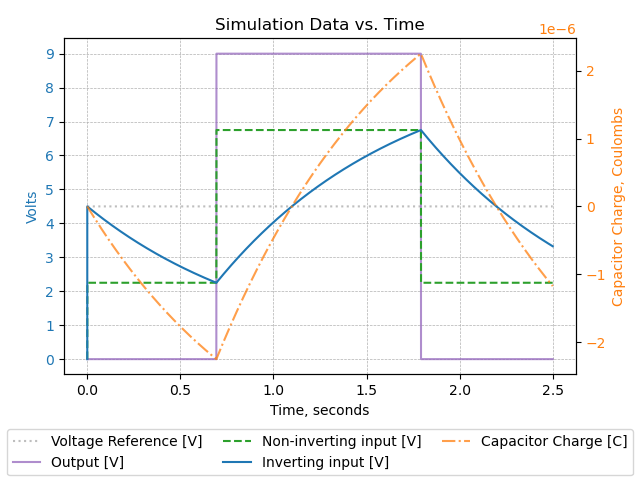
\includegraphics[width=0.65\linewidth]{assets/Simulation_2.png}
\begin{lstlisting}[basicstyle=\ttfamily,frame=tb,breaklines=true]
The circuit oscillates with a frequency of 0.455 Hz (Period = 2.197 s).
The duty cycle is 50.0% (1.099 s high / 1.099 s low).
\end{lstlisting}
\end{subfigure}\\
    
\begin{subfigure}{\textwidth}
    \centering
    \caption{Simulation Results for Entry Mode 3.2 Example}
    \label{fig:sim_3_2}
    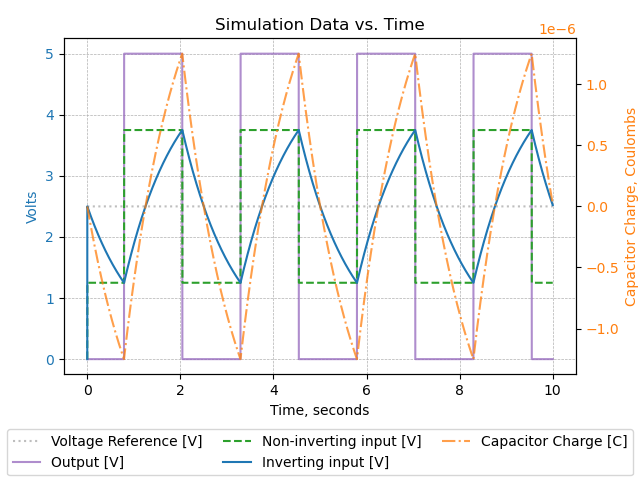
\includegraphics[width=0.65\linewidth]{assets/Simulation_3.png}
\begin{lstlisting}[basicstyle=\ttfamily,frame=tb,breaklines=true]
The circuit oscillates with a frequency of 0.400 Hz (Period = 2.500 s).
The duty cycle is 50.0% (1.250 s high / 1.250 s low).
\end{lstlisting}
\end{subfigure}
\caption{Example Graph and Console Outputs}
\label{fig:graph_ex}
\end{figure}

\clearpage
\section{Code} \label{apdx:code}
\pythonexternal[firstline=37, title={\texttt{ENGR133\_Project\_circuitSim\_ekessel.py}}]{./PythonCode/ENGR133_Project_circuitSim_ekessel.py}
\pythonexternal[firstline=38, title={\texttt{ENGR133\_Project\_circuitSim\_funcs\_ekessel.py}}]{./PythonCode/ENGR133_Project_circuitSim_funcs_ekessel.py}
\lstinputlisting[basicstyle=\ttfamily,frame=tb, title={\texttt{ENGR133\_Project\_circuitSim\_defaults\_ekessel.json}}]{./PythonCode/ENGR133_Project_circuitSim_defaults_ekessel.json}

\end{appendix}
\end{document}
